\documentclass[nooutcomes]{ximera}
\usepackage{gensymb}
\usepackage{tabularx}
\usepackage{mdframed}
\usepackage{pdfpages}
%\usepackage{chngcntr}

\let\problem\relax
\let\endproblem\relax

\newcommand{\property}[2]{#1#2}




\newtheoremstyle{SlantTheorem}{\topsep}{\fill}%%% space between body and thm
 {\slshape}                      %%% Thm body font
 {}                              %%% Indent amount (empty = no indent)
 {\bfseries\sffamily}            %%% Thm head font
 {}                              %%% Punctuation after thm head
 {3ex}                           %%% Space after thm head
 {\thmname{#1}\thmnumber{ #2}\thmnote{ \bfseries(#3)}} %%% Thm head spec
\theoremstyle{SlantTheorem}
\newtheorem{problem}{Problem}[]

%\counterwithin*{problem}{section}



%%%%%%%%%%%%%%%%%%%%%%%%%%%%Jenny's code%%%%%%%%%%%%%%%%%%%%

%%% Solution environment
%\newenvironment{solution}{
%\ifhandout\setbox0\vbox\bgroup\else
%\begin{trivlist}\item[\hskip \labelsep\small\itshape\bfseries Solution\hspace{2ex}]
%\par\noindent\upshape\small
%\fi}
%{\ifhandout\egroup\else
%\end{trivlist}
%\fi}
%
%
%%% instructorIntro environment
%\ifhandout
%\newenvironment{instructorIntro}[1][false]%
%{%
%\def\givenatend{\boolean{#1}}\ifthenelse{\boolean{#1}}{\begin{trivlist}\item}{\setbox0\vbox\bgroup}{}
%}
%{%
%\ifthenelse{\givenatend}{\end{trivlist}}{\egroup}{}
%}
%\else
%\newenvironment{instructorIntro}[1][false]%
%{%
%  \ifthenelse{\boolean{#1}}{\begin{trivlist}\item[\hskip \labelsep\bfseries Instructor Notes:\hspace{2ex}]}
%{\begin{trivlist}\item[\hskip \labelsep\bfseries Instructor Notes:\hspace{2ex}]}
%{}
%}
%% %% line at the bottom} 
%{\end{trivlist}\par\addvspace{.5ex}\nobreak\noindent\hung} 
%\fi
%
%


\let\instructorNotes\relax
\let\endinstructorNotes\relax
%%% instructorNotes environment
\ifhandout
\newenvironment{instructorNotes}[1][false]%
{%
\def\givenatend{\boolean{#1}}\ifthenelse{\boolean{#1}}{\begin{trivlist}\item}{\setbox0\vbox\bgroup}{}
}
{%
\ifthenelse{\givenatend}{\end{trivlist}}{\egroup}{}
}
\else
\newenvironment{instructorNotes}[1][false]%
{%
  \ifthenelse{\boolean{#1}}{\begin{trivlist}\item[\hskip \labelsep\bfseries {\Large Instructor Notes: \\} \hspace{\textwidth} ]}
{\begin{trivlist}\item[\hskip \labelsep\bfseries {\Large Instructor Notes: \\} \hspace{\textwidth} ]}
{}
}
{\end{trivlist}}
\fi


%% Suggested Timing
\newcommand{\timing}[1]{{\bf Suggested Timing: \hspace{2ex}} #1}




\hypersetup{
    colorlinks=true,       % false: boxed links; true: colored links
    linkcolor=blue,          % color of internal links (change box color with linkbordercolor)
    citecolor=green,        % color of links to bibliography
    filecolor=magenta,      % color of file links
    urlcolor=cyan           % color of external links
}

\title{The Graphic Details}
\author{Vic Ferdinand, Betsy McNeal, Jenny Sheldon}
\begin{document}
\begin{abstract}\end{abstract}
\maketitle


\begin{problem}
For each of the situations below, pick the graph that most reasonably
reflects the situation and the variables involved.

\begin{enumerate}
\item \label{graphicDetailsA} The daily high temperature recorded in Chicago from January to
  December

 \begin{center}
     \begin{tikzpicture}
         \draw[->](0,0)--(5,0);
         \draw[->](0,0)--(0,5);
         \node at (4, -0.2) {Month};
         \node[rotate=90] at (-0.2, 3) {Temperature};
         \draw[domain=0:5] plot (\x, {-0.4*(\x-2.5)^2+4});
         \node at (4.2, 3.4) {$A$};
         \draw[domain=0:2.5] plot (\x, {1.5+0.7*\x});
         \draw[domain=2.5:5] plot (\x, {3.25-0.7*(\x-2.5)});
         \node at (4.2, 1.3) {$C$};
         \draw plot[smooth] coordinates {(0,1.5) (1, 1.6) (2, 2.4) (2.5,2.52) (3,2.4) (4,1.6) (5,1.5)};
         \node at (3.2, 3) {$B$};
     \end{tikzpicture}
 \end{center}

\item \label{graphicDetailsB} The number of gallons of milk you can buy with $\$5$ as the cost per gallon of
  milk increases

\begin{center}
    \begin{tikzpicture}
        \draw[->](0,0)--(5,0);
        \draw[->](0,0)--(0,5);
        \node at (4, -0.2) {Cost};
        \node[rotate=90] at (-0.2, 3) {Gallons of Milk};
        \draw[domain=0:4] plot (\x, {0.2+\x});
        \node at (4.2, 4.4) {$A$};
        \draw[domain=0:4.5] plot (\x, {4.8-\x});
        \node at (4.6, 0.15) {$C$};
        \draw[domain=0.4:5] plot (\x, {2/\x});
        \node at (5.2, 0.4) {$B$};
    \end{tikzpicture}
\end{center}

\end{enumerate}
\end{problem}

\newpage


\begin{problem} \label{graphicDetails2}
Water is poured at a constant rate into the three containers shown
below. Which graph corresponds to which container?

\begin{center}
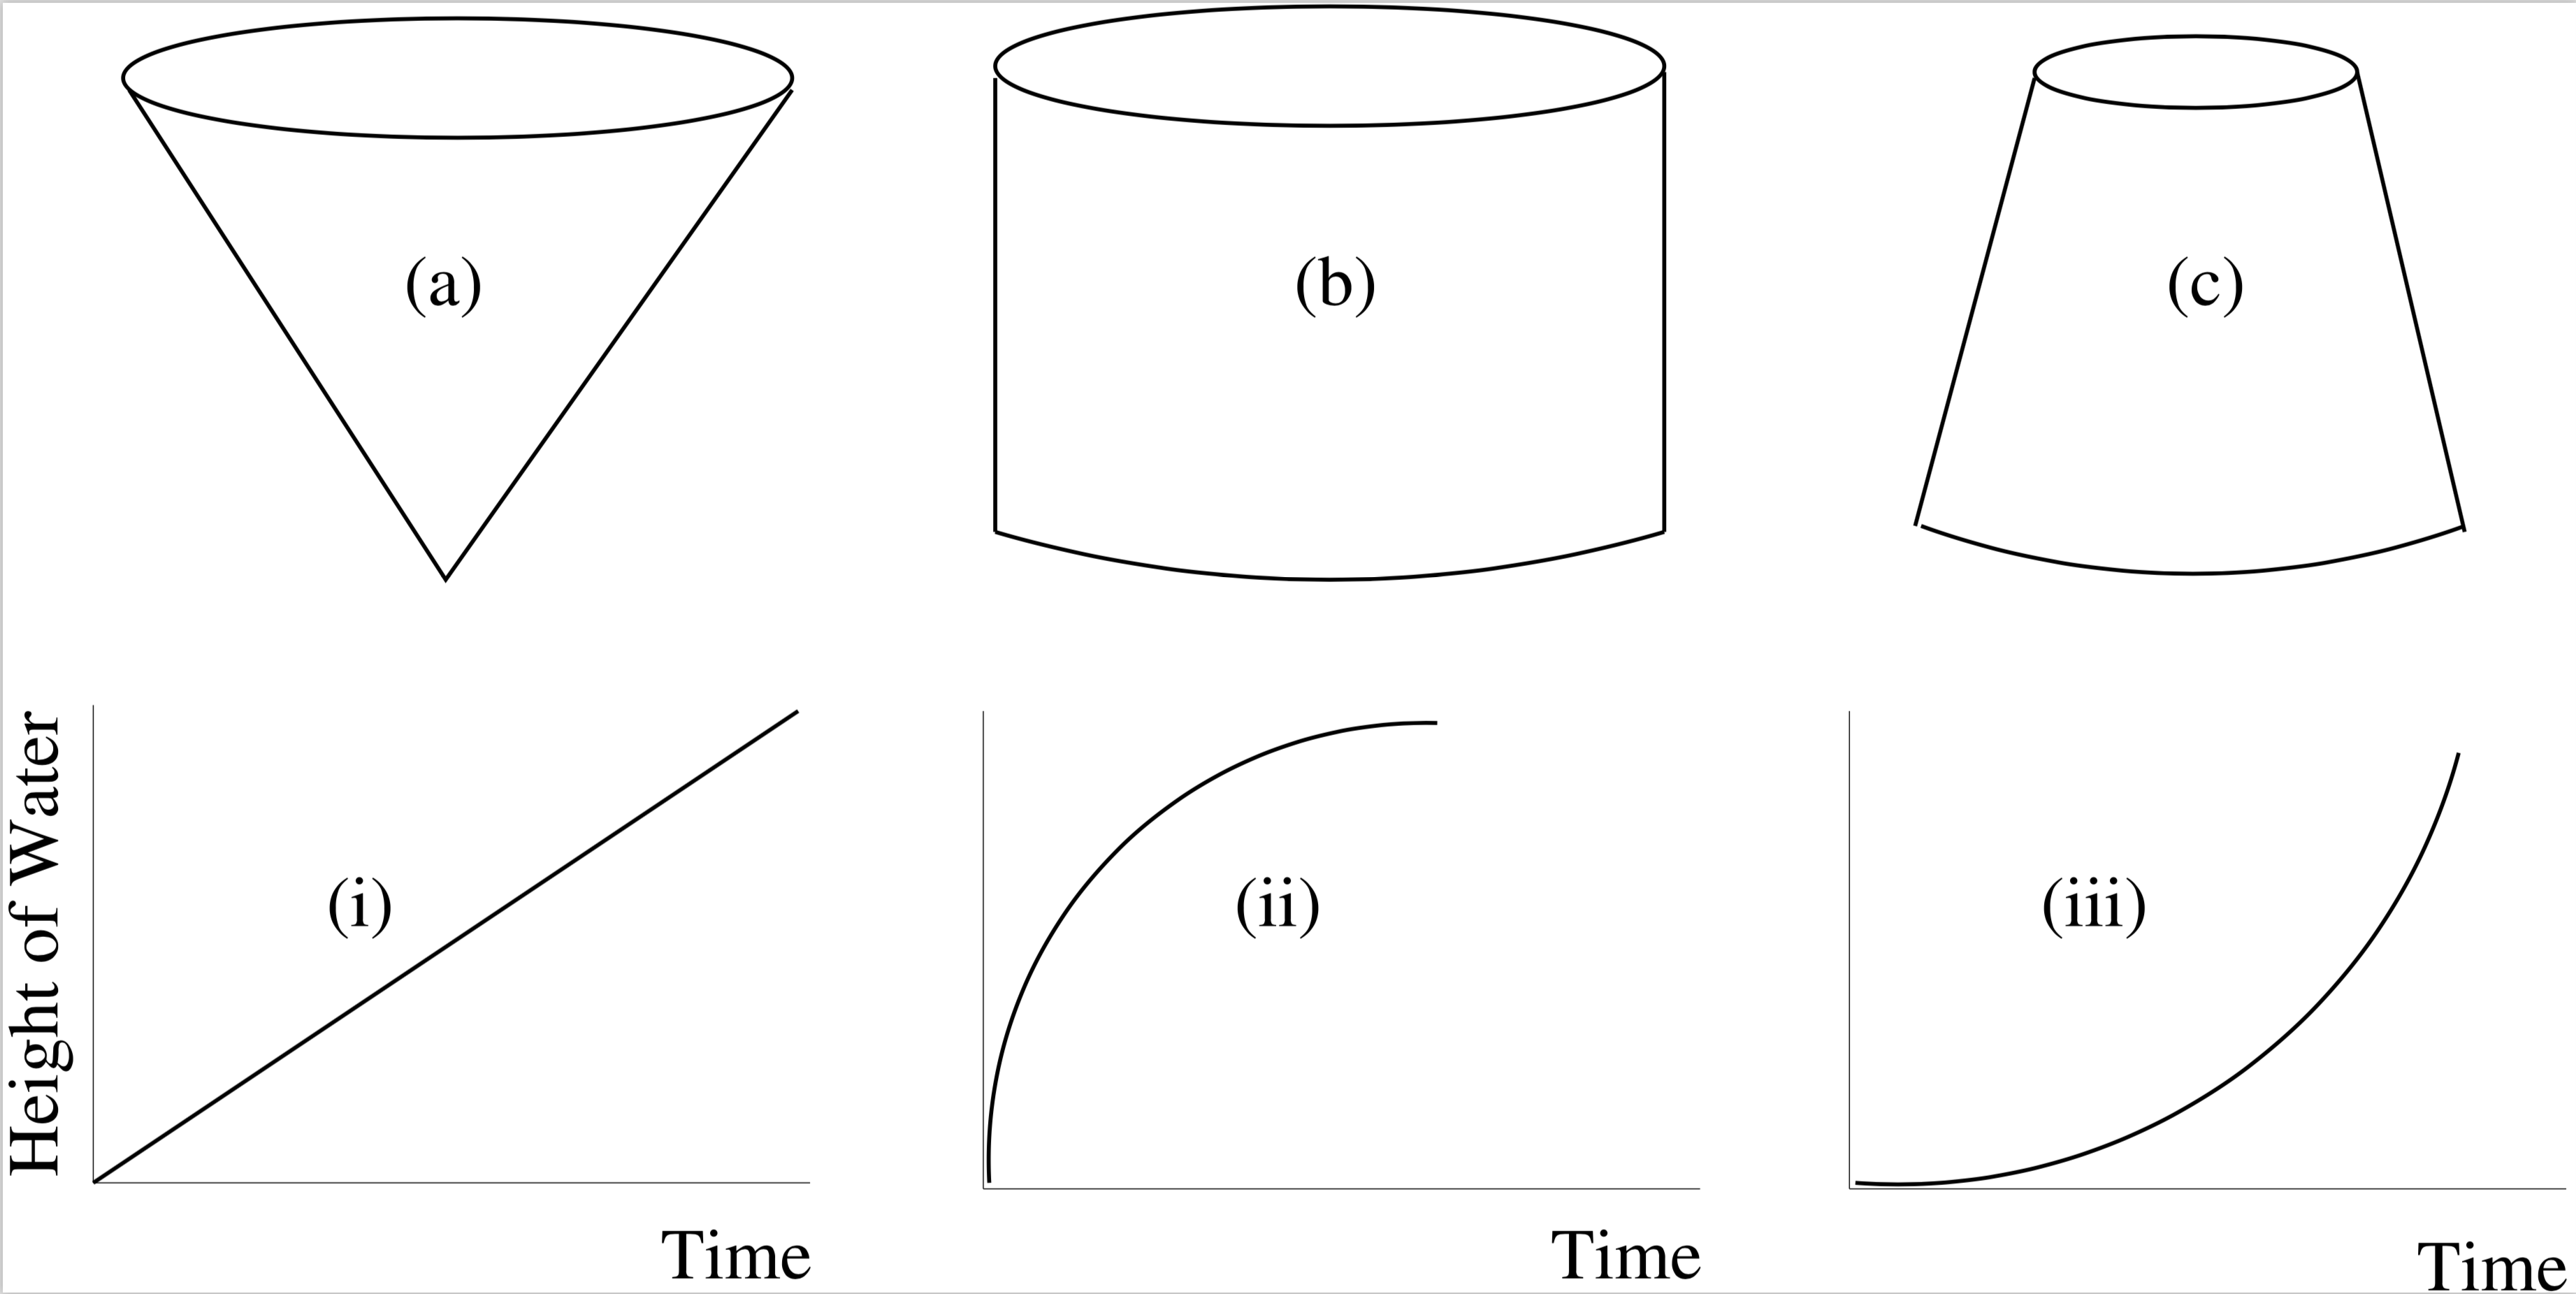
\includegraphics[width=\textwidth]{graphicDetails2.png}
\end{center}


\end{problem}

\newpage

\begin{problem} \label{graphicDetails3}
Water is poured at a constant rate into the six containers shown
below. Which graph corresponds to which container?

\begin{center}
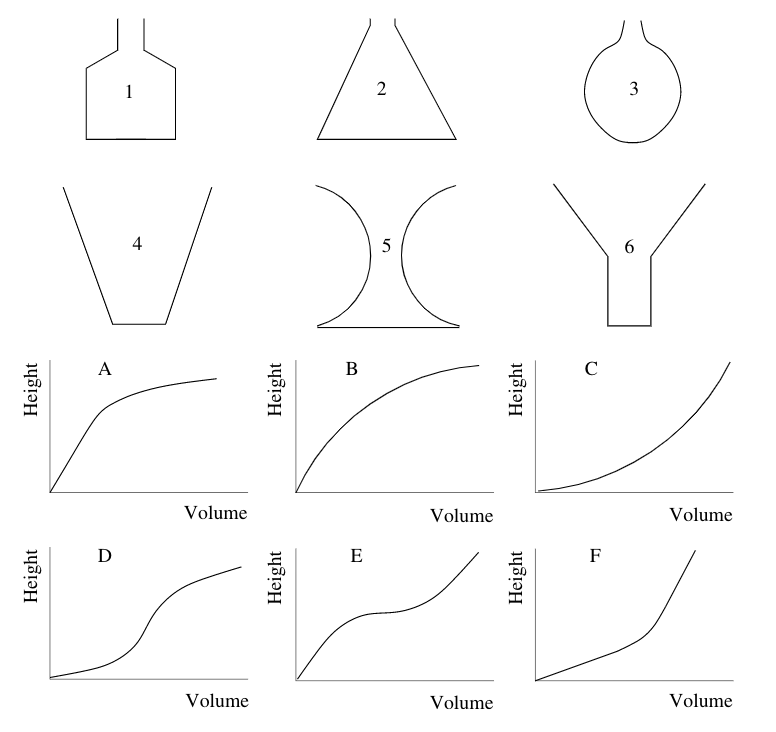
\includegraphics[width=\textwidth]{graphicDetails3.png}
\end{center}


\end{problem}

\newpage

\begin{instructorNotes}
Here we begin to inspect graphical representations of functions or expressions rather than algebraic or tabular representations.  In our course, we have already studied algebraic expressions (in the first semester) and so this activity helps students to begin to see a connection between algebra and geometry.  For us, this activity follows ``Where Are We?'' in which we discuss the coordinate system.  ``Where are We?'' also helps us connect work done using algebraic and tabular representations for arithmetic sequences in ``Gertrude Gumchewer'' and ``I Walk the Line'' with their graphs, so this activity is not the first for us where these connections have been made.  These prior activities can enrich the discussion here, but are not necessary for the activity.  The activity does assume that students understand what kind of information a graph is presenting, so discussing the coordinate system beforehand is required.

We use this activity to help students focus on reasoning about graphs to get information about a certain situation.  This can be challenging for students at first, especially if they are more used to using a formula or algorithm to gather information.

We also use this activity to focus on various details involved with graphing.  For instance, we use the activity to help students see that a graph can be dealt with locally as well as globally, focusing on individual points as well as the picture as a whole.  Students often focus more on the global story of what happens to one variable as the other variable changes, and often neglect the local case of the meaning of each point which is on (or off) the graph.  Also, we hope to focus students' attention on the meaning of each axis, and how changing that meaning changes the overall picture.



\begin{itemize}
    \item Part \ref{graphicDetailsA} and part \ref{graphicDetailsB} can spark a great deal of debate.  We often spend most of a class period hearing different student opinions and reasoning on which graph is most appropriate.
    \item Sometimes after enough debate, students have trouble agreeing on the correct answer for part \ref{graphicDetailsB}.  Plugging in some values can help.
    \item The problems in Problems \ref{graphicDetails2} and \ref{graphicDetails3} bring out the idea that it's important not only to study if a quantity increases or decreases, but how it does those things.  Students can often overlook non-linear relationships.
\end{itemize}



\timing{This usually takes an entire class period or more.  To shorten the activity we usually do only the first two problems. Another way to save time is to divide up the various parts among the groups, and have them present their solutions to the class, but this will generate a lot less discussion than we prefer.}





\end{instructorNotes}



\end{document}

